%%%%%%%%%%%%%%%%%%%%%%%%%%%%%%%%%%%%%%%%%
% Stylish Article
% LaTeX Template
% Version 2.1 (1/10/15)
%
% This template has been downloaded from:
% http://www.LaTeXTemplates.com
%
% Original author:
% Mathias Legrand (legrand.mathias@gmail.com) 
% With extensive modifications by:
% Vel (vel@latextemplates.com)
%
% License:
% CC BY-NC-SA 3.0 (http://creativecommons.org/licenses/by-nc-sa/3.0/)
%
%%%%%%%%%%%%%%%%%%%%%%%%%%%%%%%%%%%%%%%%%

%----------------------------------------------------------------------------------------
%	PACKAGES AND OTHER DOCUMENT CONFIGURATIONS
%----------------------------------------------------------------------------------------

\documentclass[fleqn,10pt]{SelfArx} % Document font size and equations flushed left

\usepackage[english]{babel} % Specify a different language here - english by default

\usepackage{lipsum} % Required to insert dummy text. To be removed otherwise

\captionsetup[figure]{justification=justified, singlelinecheck=off} 
\captionsetup[table]{justification=justified, singlelinecheck=off} 
%----------------------------------------------------------------------------------------
%	COLUMNS
%----------------------------------------------------------------------------------------

\setlength{\columnsep}{0.55cm} % Distance between the two columns of text
\setlength{\fboxrule}{0.75pt} % Width of the border around the abstract

%----------------------------------------------------------------------------------------
%	COLORS
%----------------------------------------------------------------------------------------

\definecolor{color1}{RGB}{0,0,90} % Color of the article title and sections
\definecolor{color2}{RGB}{0,20,20} % Color of the boxes behind the abstract and headings

%----------------------------------------------------------------------------------------
%	HYPERLINKS
%----------------------------------------------------------------------------------------

\usepackage{hyperref} % Required for hyperlinks
\hypersetup{hidelinks,colorlinks,breaklinks=true,urlcolor=color2,citecolor=color1,linkcolor=color1,bookmarksopen=false,pdftitle={Title},pdfauthor={Author}}

%----------------------------------------------------------------------------------------
%	ARTICLE INFORMATION
%----------------------------------------------------------------------------------------

% \JournalInfo{Journal, Vol. XXI, No. 1, 1-5, 2013} % Journal information
\JournalInfo{$ $ } % Journal information
\Archive{Pre-print} % Additional notes (e.g. copyright, DOI, review/research article)

\PaperTitle{Numerical Instabilities in Analytical Pipelines Compromise the Reliability of Network Neuroscience} % Article title

\Authors{Gregory Kiar\textsuperscript{1}, Yohan Chatelain\textsuperscript{2}, Pablo de Oliveira Castro\textsuperscript{3},
Eric Petit\textsuperscript{4}, Ariel Rokem\textsuperscript{5}, Gaël Varoquaux\textsuperscript{6},
Bratislav Misic\textsuperscript{1}, Tristan Glatard\textsuperscript{2$\dagger$},
Alan C. Evans\textsuperscript{1$\dagger$}} % Authors
\affiliation{\textsuperscript{1}\textit{Montréal Neurological Institute, McGill University, Montréal, QC, Canada}} % Author affiliation
\affiliation{\textsuperscript{2}\textit{Department of Computer Science and Software Engineering, Concordia University, Montréal, QC, Canada}} % Author affiliation
\affiliation{\textsuperscript{3}\textit{Department of Computer Science, Université of Versailles, Versailles, France}} % Author affiliation
\affiliation{\textsuperscript{4}\textit{Exascale Computing Lab, Intel, Paris, France}} % Author affiliation
\affiliation{\textsuperscript{5}\textit{Department of Psychology and eScience Institute, University of Washington, Seattle, WA, USA}} % Author affiliation
\affiliation{\textsuperscript{6}\textit{Parietal project-team, INRIA Saclay-ile de France, France}} % Author affiliation
\affiliation{$\dagger$Authors contributed equally}

\Keywords{Stability --- Reproducibility --- Network Neuroscience --- Neuroimaging} % Keywords - if you don't want any simply remove all the text between the curly brackets
\newcommand{\keywordname}{Keywords} % Defines the keywords heading name

%----------------------------------------------------------------------------------------
%	ABSTRACT
%----------------------------------------------------------------------------------------

\Abstract{The analysis of brain-imaging data requires complex and often non-linear transformations to support findings
on brain function or pathologies. And yet, recent work has shown that variability in the choices that one makes when
analyzing data can lead to quantitatively and qualitatively different results, endangering the trust in
conclusions~\cite{Glen2018-sg,botvinik2020variability,bennett2009neural,eklund2016cluster}. Even within a given method
or analytical technique, numerical instabilities could compromise
findings~\cite{Kiar2020-lb,salari2020file,Lewis2017-ll,Glatard2015-vc}. We instrumented a structural-connectome
estimation pipeline with Monte Carlo Arithmetic~\cite{Parker1997-qq,Denis2016-wo}, a technique to introduce random
noise in floating-point computations, and evaluated the stability of the derived connectomes, their
features~\cite{Betzel2018-eo,Rubinov2010-fh}, and the impact on a downstream analysis~\cite{Park2015-uj,Gupta2015-ap}.
The stability of results was found to be highly dependent upon which features of the connectomes were evaluated, and
ranged from perfectly stable (i.e. no observed variability across executions) to highly unstable (i.e. the results
contained no trustworthy significant information). The extreme range and variability in results presented here could
severely hamper our understanding of brain function in brain-imaging studies. However, it also highlights potential
paths forward, such leveraging this variance to reduce bias in estimates of brain connectivity. This paper demonstrates
that stability evaluations are necessary as a core component of typical analytical workflows.}

%----------------------------------------------------------------------------------------

\begin{document}

\flushbottom % Makes all text pages the same height
\maketitle % Print the title and abstract box
% \tableofcontents % Print the contents section
\thispagestyle{empty} % Removes page numbering from the first page

%----------------------------------------------------------------------------------------
%	ARTICLE CONTENTS
%----------------------------------------------------------------------------------------

The modelling of brain networks, called connectomics, has shaped our understanding of the structure and function
of the brain across a variety of organisms and scales over the last
decade~\cite{behrens2012human,xia2016connectomic,morgan2013not,van2016comparative,Rubinov2010-fh,Dubois2016-yr}.
In humans, these wiring diagrams are obtained \textit{in vivo} through Magnetic Resonance Imaging (MRI), and show
promise towards identifying biomarkers of disease. This can not only improve understanding of so-called
``connectopathies'', such as Alzhiemer's Disease and Schizophrenia, but potentially pave the way for
therapeutics~\cite{fornito2015connectomics,deco2014great,xie2012mapping,filippi2013assessment,van2014brain}.

However, the analysis of brain imaging data relies on complex computational methods and software pipelines. Tools are
trusted to perform everything from pre-processing tasks to downstream statistical evaluation. While these tools
undoubtedly undergo rigorous evaluation on bespoke datasets, in the absence of ground-truth this is often evaluated
through measures of reliability~\cite{Bartko1966-tl,Brandmaier2018-tk,bridgeford2020elim,Kiar2018-jt}, proxy outcome
statistics, or agreement with existing theory. Importantly, this means that tools are not necessarily of known or
consistent quality, and it is not uncommon that equivalent experiments may lead to diverging
conclusions~\cite{botvinik2020variability,Lewis2017-ll,Glatard2015-vc,salari2020file}. While many scientific
disciplines suffer from a lack of reproducibility~\cite{baker20161}, this was recently explored in brain imaging by a
$70$ team consortium which performed equivalent analyses and found widely inconsistent
results~\cite{botvinik2020variability}.

The present study approached evaluating reproducibility from a systemic perspective in which a series brain imaging
studies were numerically perturbed and the biological implications of the observed instabilities were quantified. We
accomplished this through the use of Monte Carlo Arithmetic (MCA)~\cite{Parker1997-qq}, a technique which enables
characterization of the sensitivity of a system to small perturbations. We explored the impact of perturbations through
the direct comparision of structural connectomes, the consistency of their features, and their eventual application in
a neuroscience study. Finally we conclude on the consequences of the observed instabilities and make recommendations
for future work in this area.

%------------------------------------------------
\subsection*{Graphs Vary Widely With Perturbations}
\begin{figure*}[hbt]\centering
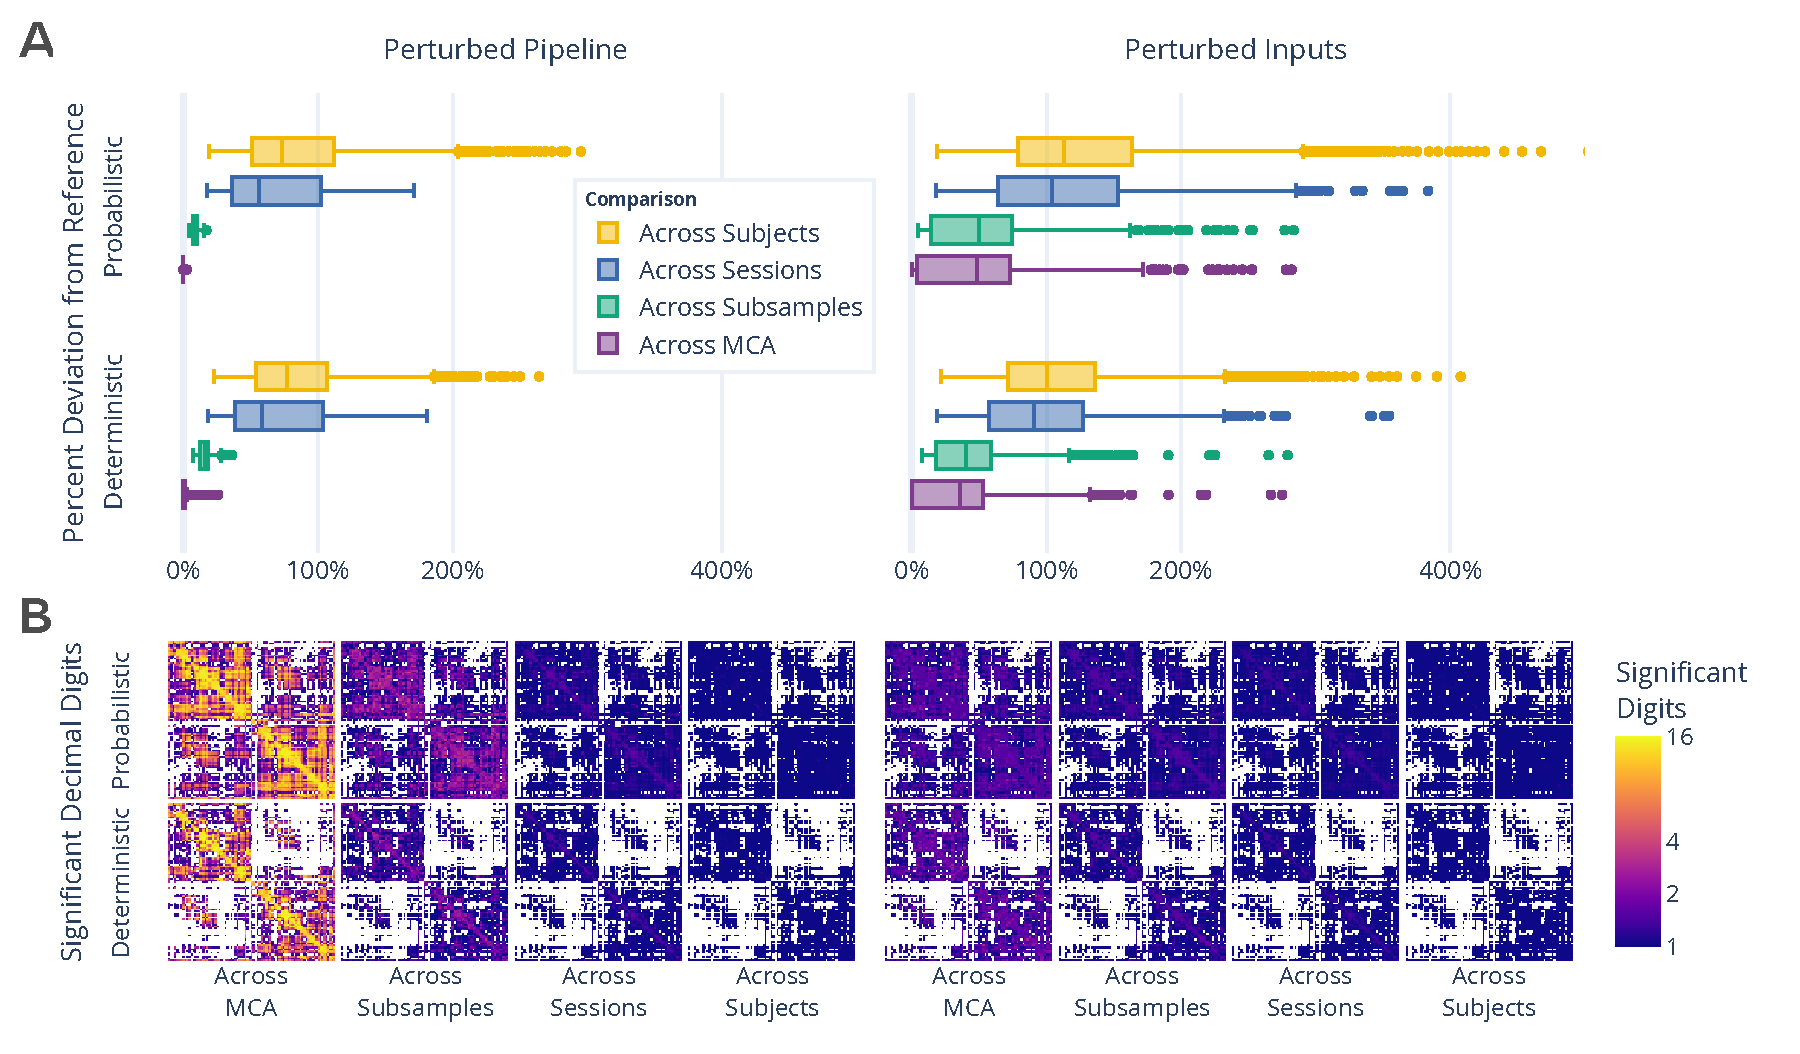
\includegraphics[width=0.98\linewidth]{figures/fig1_absolute_differences.pdf}
\caption{Exploration of perturbation-induced deviations from reference connectomes.
(\textbf{A}) The absolute deviations, in the form of normalized percent deviation from reference, shown as the
across MCA series relative to Across Subsample, Across Session, and Aross Subject variations.
(\textbf{B}) The number of significant decimal digits in each set of connectomes as obtained after evaluating the
effect of perturbations. In the case of 16, values can be fully relied upon, whereas in the case of 1 only the first
digit of a value can be trusted. Pipeline- and Input-perturbations are shown on the left and right, respectively.}
\label{fig:absolute}
\end{figure*}

{\color{red} Add single opening sentence}.
A subset of the Nathan Kline Institute Rockland Sample dataset~\cite{Nooner2012-eg} was randomly selected to contain
$25$ individuals with two sessions of imaging data, each of which was subsampled into two components, resulting in four
collections per individual. Structural connectomes were generated with canonical deterministic and probabilistic
pipelines~\cite{Garyfallidis2014-ql,Garyfallidis2012-gg} which were instrumented with MCA, mimicking computational
noise at either the inputs or throughout the pipelines~\cite{Denis2016-wo,Kiar2020-lb}. The pipelines were sampled $20$
times per collection and once without perturbations, resulting in a total of $4,200$ connectomes.

The stability of connectomes was evaluated through the deviation from reference and the number of significant digits
(Figure~\ref{fig:absolute}). The comparisons were grouped according to differences across simulations, subsampling
of data, sessions of acquisition, or subjects. While the similarity of connectomes decreases as the collections become
more distinct, connectomes generated with input perturbations show considerable variability, often reaching deviations
equal to or greater than those observed across individuals or sessions (Figure~\ref{fig:absolute}A; right). This
finding suggests that instabilities inherent to these pipelines may mask session or individual differences, limiting
the trustworthiness of derived connectomes. While both pipelines show similar performance, the probabilistic pipeline
was more stable in the face of pipeline perturbations whereas the deterministic was more stable to input perturbations
($p < 0.0001$ for all; exploratory). The stability of correlations can be found in \sref{supsec:correlation}.

The number of significant digits per edge across connectomes (Figure~\ref{fig:absolute}B) similarly decreases across
groups. While the cross-MCA comparison of connectomes generated Pipeline Perturbations show nearly perfect precision
for many edges (approaching the maximum of $15.7$ digits for $64$-bit data), this evaluation uniquely shows
considerable drop off in performance across data subsampling (average of $< 4$ digits). Input Perturbations show no
more than an average of $3$ significant digits across all groups. Significance across individuals did not exceed a
single digit per edge in any case, indicating that only the magnitude of edges in groupwise average connectomes can be
trusted. The combination of these results with those presented in Figure~\ref{fig:absolute}A suggests that while
specific edge weights are largely affected by instabilities, macro-scale network topology is stable.

\subsection*{Subject-Specific Signal is Amplified While Artifacts Are Reduced}
\begin{table*}[ht]\centering
\caption{The impact of instabilities evaluated through the separability of the dataset based on simulation, subsample,
session, and subject (reported as mean~$\pm$~standard deviation Discriminability). While a perfectly reliable dataset
would be represented by a score of $1.0$, the chance performance is $1 /$the number of classes. In the case of
Hypothesis 1, the evaluation of similarity across individuals, the chance performance is $0.04$. In the case of
Hypotheses 2 and 3, the evaluation of similarity across sessions or subsamples, respectively, the chance performance is
$0.5$. The alternative hypothesis, indicating significant separation across groups, is accepted for all experiments,
with $p < 0.005$.}
\vspace{5pt}
% \fcolorbox{color1}{white}{%
% \parbox{\textwidth-2\fboxsep-2\fboxrule}{\centering
%   \colorbox{color2!10}{
%     \parbox{\textwidth-4\fboxsep-2\fboxrule}{

\begin{tabular}{llll|ll|ll|ll}
  &  &  &  &  \multicolumn{2}{l|}{\textbf{Reference Execution}} & \multicolumn{2}{l|}{\textbf{Perturbed Pipeline}} &  \multicolumn{2}{l}{\textbf{Perturbed Inputs}} \\
Exp. & Subj. & Sess. & Samp. & Det. &  Prob. &  Det. &    Prob. &     Det. &    Prob. \\
% Exp. & Subj. & Sess. & Dirs. & Sims. &     Discrim. (D) &    Discrim. (P) &     Discrim. (D) &    Discrim. (P) \\
\hline
1.1        &          All &      All &          1 &  $ 0.64 \pm 0.00 $ &  $ 0.65 \pm 0.00 $  &  $ 0.82 \pm 0.00 $ &  $ 0.82 \pm 0.00 $ &  $ 0.77 \pm 0.00 $ &  $ 0.75 \pm 0.00 $ \\
1.2        &          All &        1 &        All &  $ 1.00 \pm 0.00 $ &  $ 1.00 \pm 0.00 $ &  $ 1.00 \pm 0.00 $ &  $ 1.00 \pm 0.00 $ &  $ 0.93 \pm 0.02 $ &  $ 0.90 \pm 0.02 $ \\
1.3        &          All &        1 &          1 &        &  &  $ 1.00 \pm 0.00 $ &  $ 1.00 \pm 0.00 $ &  $ 0.94 \pm 0.02 $ &  $ 0.90 \pm 0.02 $ \\
& & & & & & & & & \vspace{-5pt}\\
2.4        &            1 &      All &        All &  $ 1.00 \pm 0.00 $ &  $ 1.00 \pm 0.00 $  &  $ 1.00 \pm 0.00 $ &  $ 1.00 \pm 0.00 $ &  $ 0.88 \pm 0.12 $ &  $ 0.85 \pm 0.12 $ \\
2.5        &            1 &      All &          1 &        &  &  $ 1.00 \pm 0.00 $ &  $ 1.00 \pm 0.00 $ &  $ 0.89 \pm 0.11 $ &  $ 0.84 \pm 0.12 $ \\
& & & & & & & & & \vspace{-5pt}\\
3.6        &            1 &        1 &        All &         &  &  $ 0.99 \pm 0.03 $ &  $ 1.00 \pm 0.00 $ &  $ 0.71 \pm 0.07 $ &  $ 0.61 \pm 0.05 $ \\
\end{tabular}


%     }
%   }
% }%
% }%

\label{tab:discrim}
\end{table*}

We assessed the reproducibility of the dataset through mimicking and extending a typical test-retest
experiment~\cite{bridgeford2020elim} in which the similarity of similar samples across multiple measurements were
compared to distinct samples in the dataset (Table~\ref{tab:discrim}). The ability to separate connectomes across
subjects (Experiments 1.1, 1.2, and 1.3) is an essential prerequisite for the application of brain imaging towards
identifying individual differences~\cite{Dubois2016-yr}. In experiment 1.1, we observe that the dataset is separable
with a score of $0.64$ and $0.65$ ($p < 0.001$; optimal score: $1.0$; chance: $0.04$) without any instrumentation.
However, we can see that inducing instabilities through MCA improves the reliability of the dataset to over $0.75$ in
each case ($p < 0.001$ for all), significantly higher than without instrumentation or greater in ($p < 0.005$ for all).
This result impactfully suggests the utility of perturbation methods for synthesizing robust and reliable individual
estimates of connectivity, serving as a cost effective and context-agnostic method for dataset augmentation.

While the separability of individuals is essential for the identification of brain networks, this modelling is
similarly reliant on network similarity across equivalent acquisitions (Experiments 2.4, 2.5). In this case,
connectomes were grouped based upon session, rather than subject, and the ability to distinguish one session from
another was computed within-individual and aggregated. Both the unperturbed and pipeline perturbation settings
perfectly preserved differences between cross-sectional session with a score of $1.0$ ($p < 0.005$; optimal score:
$0.5$; chance: $0.05$). However, while still significant relative to chance (score: $0.85$ and $0.88$; $p < 0.005$ for
both), input perturbations lead to significantly lower separability of the dataset ($p < 0.005$ for all). This
reduction of the difference between sessions of data within individuals suggests that increased variance caused by
input perturbations reduces the impact of non-biological acquisition-dependent bias inherent in the brain graphs.

Though the previous sets of experiments inextricably evaluate the interaction between the dataset and tool, the use of
subsampling allowed for characterizing the separability of networks sampled from within a single acquisition
(Experiment 3.6). While this experiment could not be evaluated using reference executions, the executions performed
with pipeline perturbations showed near perfect separation between subsamples, with scores of $0.99$ and $1.0$
($p < 0.005$; optimal: $0.5$; chance: $0.5$). Given that there is no variability in data acquisition or preprocessing
that contributes to this reliable identification of scans, the separability observed in this experiment may only be due
to instability or bias inherent to the pipelines. The high variability introduced through input perturbations
considerably lowered the reliability towards chance (score: $0.71$ and $0.61$; $p < 0.005$ for all), further supporting
this as an effective method for obtaining lower-bias estimates of individual connectivity.

In all cases the induced perturbations showed an amplification of meaningful biological signal alongside a reduction of
off-target bias across all experiments. This result highlights that stability evaluation can be used not only to
identify instabilities and variance within pipelines, but that the observed variance may be leveraged for the
generation of robust distributions of results.

{\color{red} unedited past here}.

\subsection*{Distributions of Graph Statistics Are Reliable, Individual Statistics Are Not}
\begin{figure*}[bt!]\centering
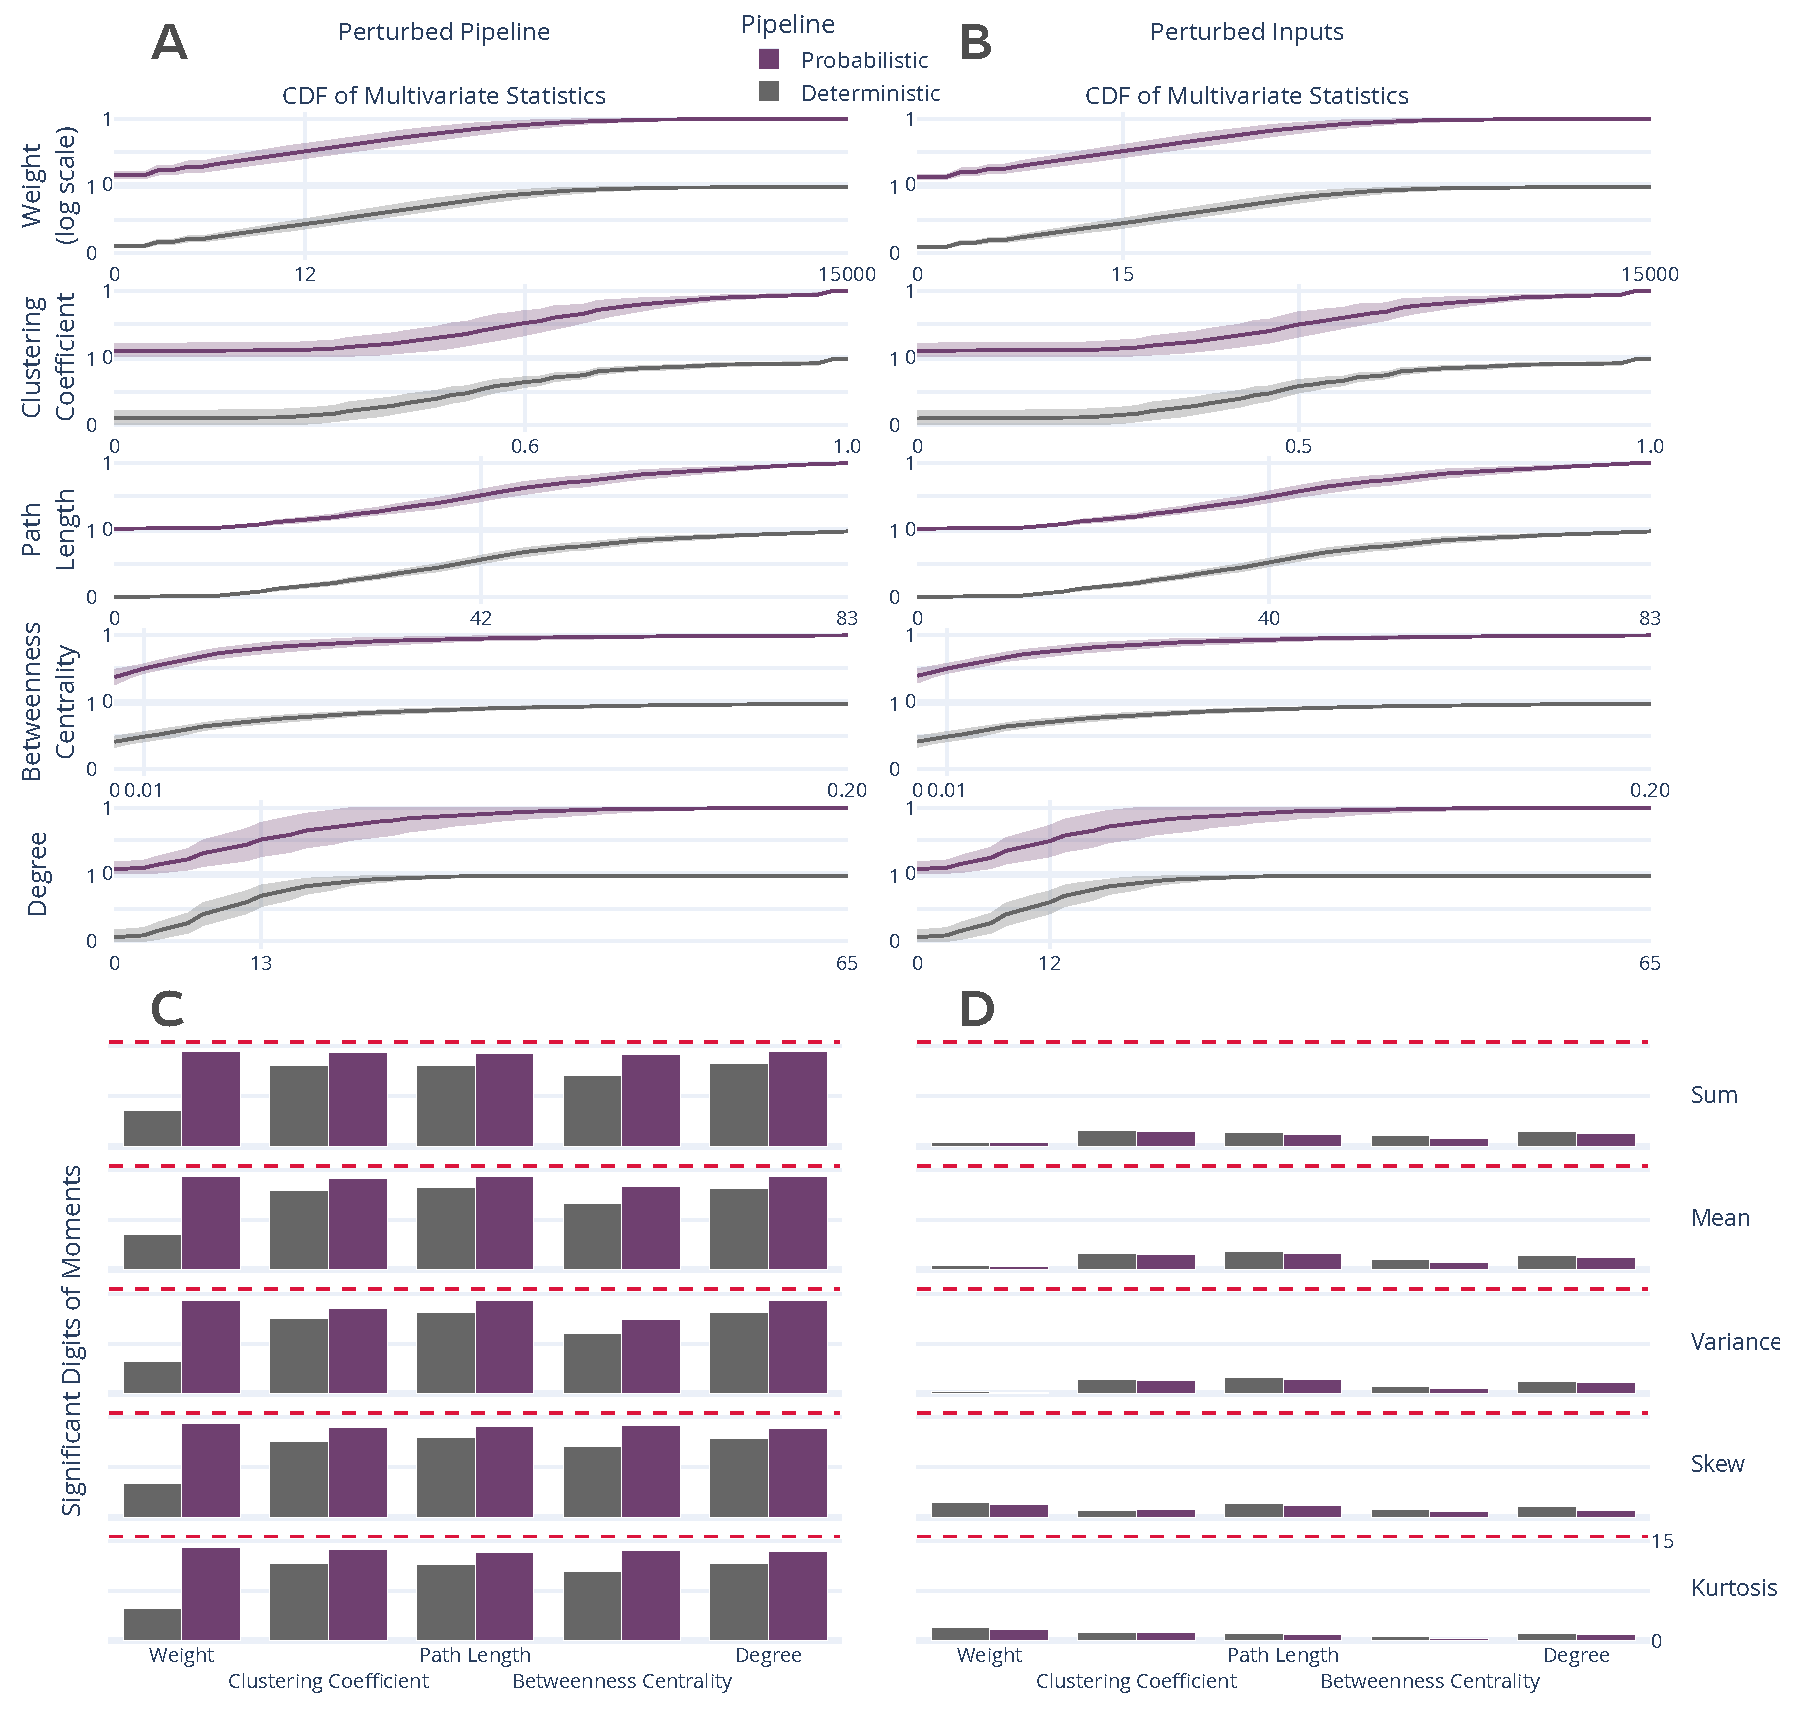
\includegraphics[width=\linewidth]{figures/fig2_multivariate_differences.pdf}
\caption{Distribution and stability assessment of multivariate graph statistics. (\textbf{A}, \textbf{B}) The
cumulative distribution functions of multivariate statistics across all subjects and perturbation settings. There was
no significant difference between the distributions in A and B. (\textbf{C}, \textbf{D}) The number of significant
digits in the first five moments of each statistic across perturbations. The dashed red line refers to the maximum
possible number of significant digits.}
\label{fig:multivar}
\end{figure*}

\begin{itemize}
\item define measures and cite their common use
\item define comparison of distributions and discuss implication (distributions are stable)
\item define comparison of moments (individual statistics are unstable)
\item summarize impact (group-wise distributions should be relied upon rather than individual differences)
\end{itemize}

Connectomes are often summarized by lower-dimensional statistics more suitable for numerous analytical
methods~\cite{Rubinov2010-fh}. Figure~\ref{fig:multivar} explores the stability of these graph-theoretical metrics
computed from the perturbed graphs, including weight, clustering coefficient, path length, betweenness centrality, and
degree. Due to the variable length of the edgewise statistics, cumulative density functions for each statistic were
evaluated over a fixed range and the mean density and associated standard error were computed for each bin
(Figures~\ref{fig:multivar}A and ~\ref{fig:multivar}B), with the distributions' minimum, median, and maximum values
denoted on each x-axis. There was no significant difference in distributions observed for each statistic across the two
perturbation settings. The first 5 moments of these statistics within individuals as observed with Pipeline
Perturbations (Figure~\ref{fig:multivar}C) were stable with more than $10$ significant digits with the exception of
edge weight when using the deterministic pipeline. In the case of all statistics, the probabilistic pipeline was more
stable than the deterministic pipeline ($p < 0.0001$; exploratory). In stark contrast, these moments were highly
unstable in the face of Input Perturbations (Figure~\ref{fig:multivar}D), in which no measure had more than $5$
significant digits of information, and several moment and statistic pairs had less than a single significant digit,
such as the variance in edge weight or the kurtosis of betweenness centrality. In general, there was not a strong
relationship between the order of the moment and its stability. A similar analysis was performed for univariate
statistics in \sref{supsec:univar}.

The large discrepancy between the stability of individual estimates in these settings versus the similarity of
aggregated CDFs suggests that while individual estimates are unstable, the comparison between aggregates or groups may
be considered much more reliable.

\subsection*{The Strength of Brain-Behaviour Relationships is Eroded}

\begin{figure*}[ht]\centering
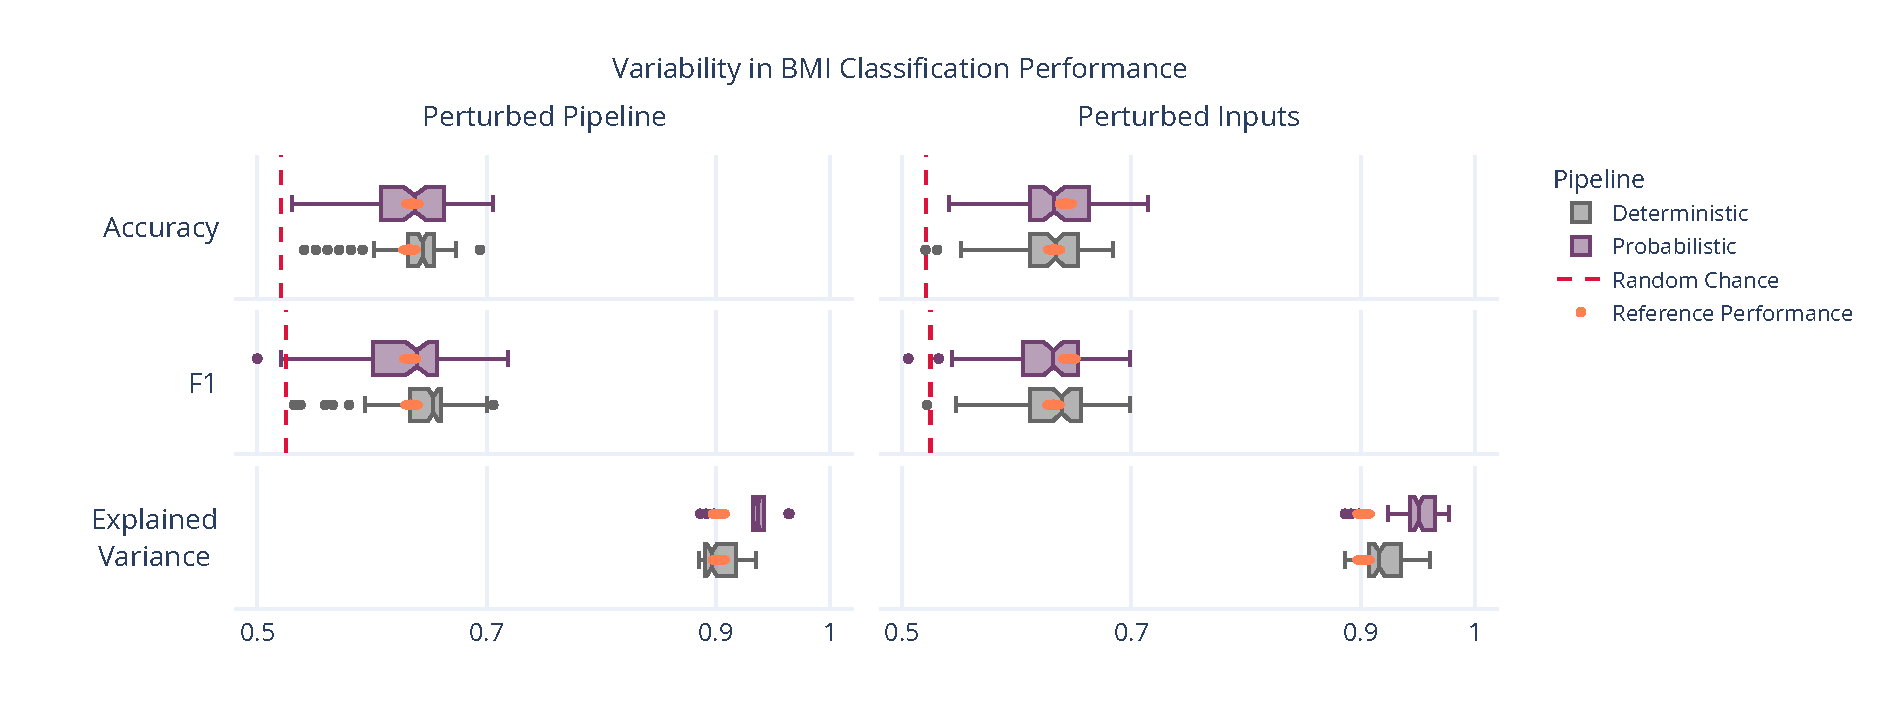
\includegraphics[width=\linewidth]{figures/fig3_bmi_classification.pdf}
\caption{Observed variability in BMI classification. Training and Test sets were sampled from the MCA-generated dataset
such that a single observation of each individual was present in each sampling. This sampling was performed 20 times,
and each dataset was used to train a classifier with each of 2, 5, 10, and N-fold cross validation, and the shown
metrics are the average across each of these training paradigms. The dashed red lines indicate random-chance
performance, and the orange dots show the performance using the reference executions.}
\label{fig:bmi}
\end{figure*}

\begin{itemize}
\item define classification task and cite justification
\item state reference performance and distribution of perturbed performances
\item summarize impact (the strength of biological signal is highly unstable and erodes confidence in models of brain
behaviour relationships)
\end{itemize}

While the variability of explicit features of connectomes was summarized above, these networks are commonly-used as
inputs to machine learning models. Here, connectomes were projected into a low dimensional space using PCA and then
input a logistic regression classifier (Figure~\ref{fig:bmi}). The number of principal components was selected as the
minimum number of components required to capture 90\% of the variance in the reference set; this resulted in $20$
components. Using the reference performance, i.e. that using only unperturbed graphs (Figure~\ref{fig:bmi}; orange
overlay), the classification accuracies were $0.635$ and $0.628$, and the F1 scores were $0.636$ and $0.630$ for data
derived using the deterministic and probabilistic pipelines, respectively, with the average explained variance at 90\%
in both cases. The random chance performance for these evaluations measures were $0.521$ and $0.519$, respectively
(Figure~\ref{fig:bmi}; dashed red line).

When performing this analysis using sampled instances of the perturbed dataset across both pipelines and perturbation
methods, the portion of explained variance in the sample with $20$ components ranged from $0.886$ -– $0.978$. The
classification accuracy ranged from $0.520$ – $0.716$ and the F1 score ranged from $0.510$ -– $0.725$. These results
range from at or below random chance performance, to considerable accuracy that outperforms that obtained using the
reference dataset.

\subsection*{Discussion}

This paper explores the impact of perturbing a structural connectome estimation pipeline with small amounts of noise, on the order of machine error. These impacts were explored through three distinct comparisons of the derived connectomes: comparison of networks directly, comparison of commonly used network features, and comparison of the performance of a downstream analytical task. In each analysis we found considerable variability across the perturbed executions. Perhaps more notably, we found that the variability was itself highly variable across data, perturbation, feature, and measure. In each exploration we found that the stability of results ranged from nearly perfectly trustworthy (i.e. no variation or fully significant) to untrustworthy often to the level of only two or three significant digits of information, and occasionally with no significant digits at all.

The adoption of Monte Carlo Arithmetic for this application allowed for not only the characterization of concrete measures of stability within individual samples, such as the number of significant digits in edges of a connectome or a derived statistic, but allowed these values to be situated with respect to other biologically meaningful sources of variability such as cross-session or cross-individual variation. Importantly, the evaluation of the stability of graphs in the cross-direction subsampling setting would not have been possible without either a realistic noise model or a simulation technique similar to MCA in which multiple results are derived from a single sample of input data.


One emergent theme across all analyses was that Input Perturbations led to considerably less stable than Pipeline Perturbations, confirming observations in [10]. However, the distributions of connectomes and their statistics were not distinct from one another. This is strong support for the groupwise evaluation of graph statistics over the use of individual estimates for applications in brain imaging.

The difference in stability between the two instrumentations opens the door for many avenues for future work. The two implementations of MCA were determined, for practical reasons, as the boundary between software libraries; Pipeline Perturbations included a much more complete instrumentation, resulting in a higher density of perturbations. We hypothesize that the increased density of Pipeline Perturbations allow for the law of large numbers to mask critically unstable points within the pipeline, whereas errors introduced in the Input Perturbation implementation are allowed to propagate longer before correction. This question is non-trivially answered as understanding the true density of "coverage" of an arbitrary pipeline is impossible without direct assessment. Once coverage is evaluated for a given tool, instrumentations perturbing different degrees of the pipeline have potential to shed light on the relationship between the magnitude, frequency, and density of perturbations on the observed stability, as well as reduce the computational burden of MCA.

Another observation which became apparent across the analyses was that variability changed significantly based on measure or resolution. For instance, graphs generated with Input Perturbations were perceived to be significantly more similar to one another when compared with correlation compared to percent deviation or significant digits measures. Importantly, this does not imply correlation as a superior statistic or means for the comparison of graphs, but just that it is more robust, or less sensitive, under these circumstances. If an initial evaluation of these graphs were performed solely using correlation, it would perhaps lead the researcher to believe that their measures are perfectly stable. However, if their downstream analysis depended on one of the statistics demonstrated through Figures 2 and 3 to be highly unstable, this assumption would be incorrect. What this suggests is rather that the stability of any measures intended to be used in an analysis should be quantified, as the stability of one measure cannot be perfectly inferred from another.

A Limit in Detection of Individual Differences

The finding that individually derived network statistics were unreliable in the Input Perturbations setting despite resulting in no aggregated change has important implications on applications of connectomics. This finding bounds the success of studying individual differences, a central objective in brain imaging (Dubois and Adolphs 2016). More specifically, the relationships found between pheno/genotypic data and these statistics or connectomes in general will be limited by the reliability of the statistics themselves. While this has obvious implications in machine-learning applications such as the classification task studied above, this limitation extends to hypothesis testing as well. Though the result of an individual comparison in a hypothesis test will have a reported false-positive rate, the accuracy of this rate is dependent on the reliability of the sample used. For instance, if MCA were performed and each single observation of a highly unstable sample were used in a hypothesis test, the true false positive rate would be a combination of the variability in the results of that hypothesis test and the reported rate under the parameters of the model. Without a repeated-measure setting such as MCA, it is impossible to empirically estimate the reliability of the samples used in hypothesis testing, meaning that the reliability of accepted hypotheses is unknown, regardless of the reported false positive rate. In fact, it is a virtual certainty that the true false positive rate for a given hypothesis exceeds that reported by the terminal test simply as a result of numerical instabilities.

Eroding the Biological Plausibility of Derived Connectomes

One important insight uniquely provided by the classification task performed above is with regards to the biological plausibility of derived connectomes. While previous analyses explored the variability of the connectomes or their features, with the exception of comparisons to cross-subject variability these values were not situated with respect to meaningful biological differences. The results shown here demonstrate that our MCA-based perturbations not only distort results, but do so while retaining meaningful signal rather than merely degrading our estimates. This analysis allows us to demonstrate considerable variability in classification performance, in which we observe the reference execution to be approximately centered in the distribution of results. Critically, while MCA perturbations are data-agnostic, this result is strong evidence in favour of the quality of derived connectomes observed using MCA, suggesting that it can be used effectively in conjunction with, or in lieu of, context-aware noise models, as is often the case in brain imaging. 

Shortcomings and Future Questions

A limitation of the approach presented in this paper is the difficulty of instrumentation for arbitrary libraries with MCA. This is non-trivial for many tools due to a dependence on recompilation under specific settings. For this reason all modeling pipelines tested here were constructed using Dipy (Garyfallidis et al. 2014), a canonical Python library which provides accessible implementations of commonly-used algorithms in tractography. Pre-processing was not perturbed in these experiments. Other work has shown that linear registration is sensitive to minor perturbations, a prerequisite and core piece of many elements of pre-processing such as motion correction and alignment [8]. In practice, this suggests that the instabilities observed here would be compounded with those introduced in pre-processing.

Additionally, the analyses performed in this paper were using a single dataset and a single set of similar analysis pipelines. While the conclusions stated here have been observed in other modalities and tools used in neuroimaging through other means, the nature of this work makes it impossible to know how reliable other tools or datasets are when perturbed and evaluated similarly. Extending this work to both typical fMRI and structural MRI workflows is of interest, and the topic of future projects.

This paper also does not address methodological flexibility or compare this to the observed instability. As was demonstrated by NARPS in a task-based fMRI analysis setting [26], there exists a nearly boundless space of possible combinations of tools scientists could choose to compose their pipelines. As a result, research groups often end up using unique processing pipelines and infrastructures, which may lead to divergent conclusions even in the face of modeling identical datasets. The evaluation performed here does not compare observed the impact of MCA-induced instabilities to variability of this sort. In fact, these studies explore instability at the opposite ends of the analysis spectrum: from human introduced variability in the conceptualization and realization of an analysis workflow on the one hand, down to the unavoidable error implicit in the digital representation of data. It is of extreme interest to combine these approaches and explore the interaction of these scientific degrees of freedom with effects from software implementations, libraries, and parametric choices.

Finally, it is important to state explicitly that the work presented here does not invalidate the analytical pipelines but merely state that many studies are accompanied by an unknown degree of uncertainty due to machine-introduced errors. The desired outcome of this paper is to motivate a shift in scientific computing – particularly in neuroimaging – towards a paradigm which values the explicit evaluation of the trustworthiness of claims alongside the claims themselves.

{\color{orange}Notes\\\\
You could mention that instabilities affect not only the topology, but the geometry of reconstructed networks.

It means that we are, as a field, overconfident in numerical stability, and that in a typical setting this would lead
to wrong conclusions. Or am I over-stating it? Because if that's the case, it needs to be unequivocally stated here.
And in the abstract. And maybe also in the title of the article. this amount of numerical noise is to be expected in
typical settings, not only in MCA. Is that correct? And that has implications for inferences in the typical setting.
}

%----------------------------------------------------------------------------------------
%	REFERENCE LIST
%----------------------------------------------------------------------------------------
\phantomsection
\bibliographystyle{IEEEtran}
{\footnotesize \bibliography{impact-of-instability}}

\section*{Methods}
\begin{equation}
\cos^3 \theta =\frac{1}{4}\cos\theta+\frac{3}{4}\cos 3\theta
\label{eq:refname2}
\end{equation}

\lipsum[10] % Dummy text

\begin{enumerate}[noitemsep] % [noitemsep] removes whitespace between the items for a compact look
\item First item in a list
\item Second item in a list
\item Third item in a list
\end{enumerate}

\lipsum[14] % Dummy text

\begin{itemize}[noitemsep] % [noitemsep] removes whitespace between the items for a compact look
\item First item in a list
\item Second item in a list
\item Third item in a list
\end{itemize}

%------------------------------------------------
\phantomsection
\subsection*{Author Contributions}
GK was responsible for the experimental design, data processing, analysis, interpretation, and the majority of writing.
All authors contributed to the revision of the manuscript. YC, POC, and EP were responsible for MCA tool development
and software testing. AR, GV, and BM contributed to experimental design and interpretation. TG contributed to
experimental design, analysis, and interpretation. TG and ACE were responsible for supervising and supporting all
contributions made by GK. The authors declare no competing interests for this work.

\subsection*{Acknowledgments} 
This research was financially supported by the Natural Sciences and Engineering Research Council of Canada (NSERC)
(award no. CGSD3-519497-2018). This work was also supported in part by funding provided by Brain Canada, in partnership
with Health Canada, for the Canadian Open Neuroscience Platform initiative.

\subsection*{Additional Information}
Supplementary Information is available for this paper. Correspondence and requests for materials should be addressed to
Tristan Glatard at \url{tristan.glatard@concordia.ca}.

%----------------------------------------------------------------------------------------
\beginsupplement

\clearpage
\section{Graph Correlation}
\label{supsec:correlation}
The correlations between observed graphs (Figure 1B) across each grouping follow the same trend to percent deviation.
However, notably different from percent deviation, there is no significant difference in the correlations between
Pipeline or Input instrumentations. By this measure, the probabilistic pipeline is more stable in all cross-MCA and
cross-directions except for the combination of Input Perturbation and cross-MCA (p < 0.0001 for all; exploratory).

\begin{figure}[ht]\centering
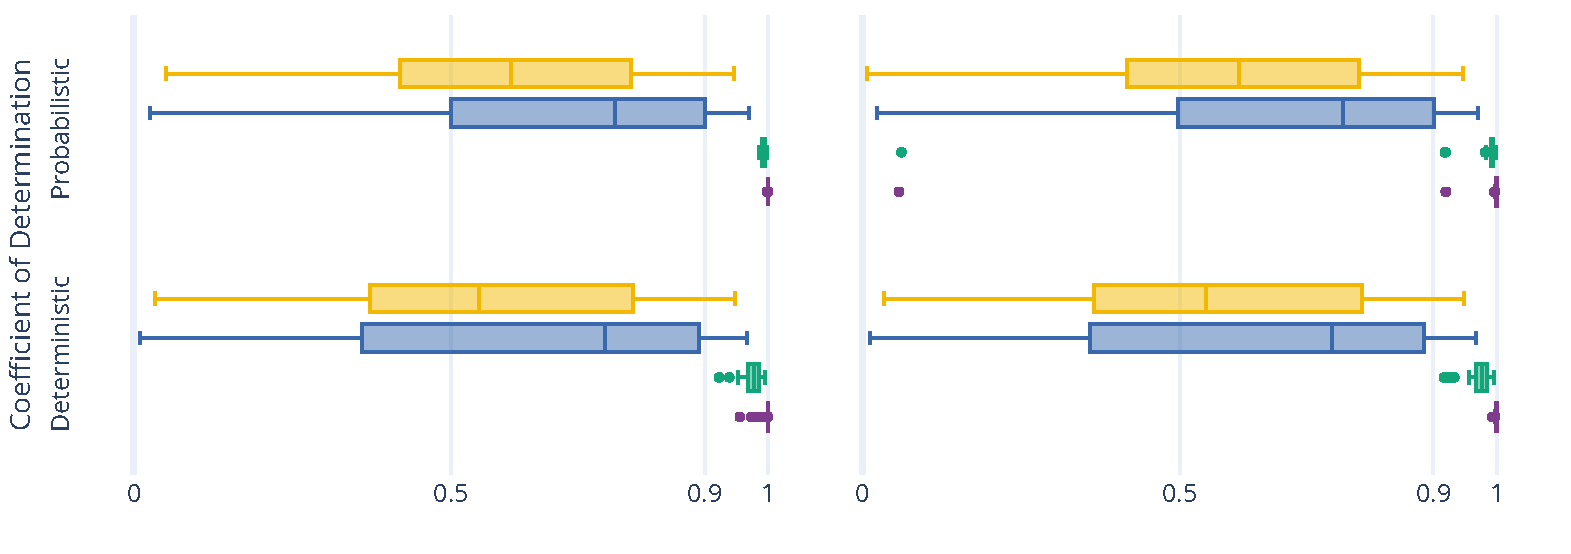
\includegraphics[width=\linewidth]{figures/figS1_correlation_differences.pdf}
\caption{The correlation between perturbed connectomes and their reference.}
\label{fig:correlation}
\end{figure}

\clearpage
\section{Univariate Graph Statistics}
\label{supsec:univar}

Figure 2 explores the stability of these graph-theoretical metrics computed from the perturbed graphs, including
modularity, global efficiency, assortativity, average path length, and edge count. When aggregated across individuals
and perturbations, the distributions of these statistics (Figures 2A and 2B) show no significant differences between
perturbation methods for either deterministic or probabilistic pipelines. However, when quantifying the stability of
these measures across connectomes derived from a single session of data, the two perturbation methods show considerable
differences. The number of significant digits in univariate statistics for Pipeline Perturbation instrumented
connectome generation exceeded 11 digits for all measures except modularity, which contained more than 4 significant
digits of information (Figure 2C). When detecting outliers from the distributions of observed statistics for a given
session, the false positive rate (using a threshold of p = 0.05) was approximately 2\% for all statistics with the
exception of modularity which again was less stable with an approximately 10\% false positive rate. The probabilistic
pipeline is significantly more stable than the deterministic pipeline (p < 0.0001; exploratory) for all features
except modularity. When similarly evaluating these features from connectomes generated in the Input Perturbation
setting, no statistic was stable with more than 3 significant digits or a false positive rate lower than nearly 6\%
(Figure 2D). The deterministic pipeline was more stable than the probabilistic pipeline in this setting (p < 0.0001;
exploratory).

Two notable differences between the two perturbation methods are, first, the uniformity in the stability of the
statistics, and second, the dramatic decline in stability of individual statistics in the Input Perturbation setting
despite the consistency in the overall distribution of values. It is unclear at present if the discrepancy between the
stability of modularity in the Pipeline Perturbation context versus the other statistics suggests the implementation of
this measure is the source of instability or if it is implicit to the measure itself. The dramatic decline in the
stability of features derived from Input Perturbed graphs despite no difference in their overall distribution both
shows that while individual estimates may be unstable the comparison between aggregates or groups may be considered
much more reliable.

\begin{figure}[ht]\centering
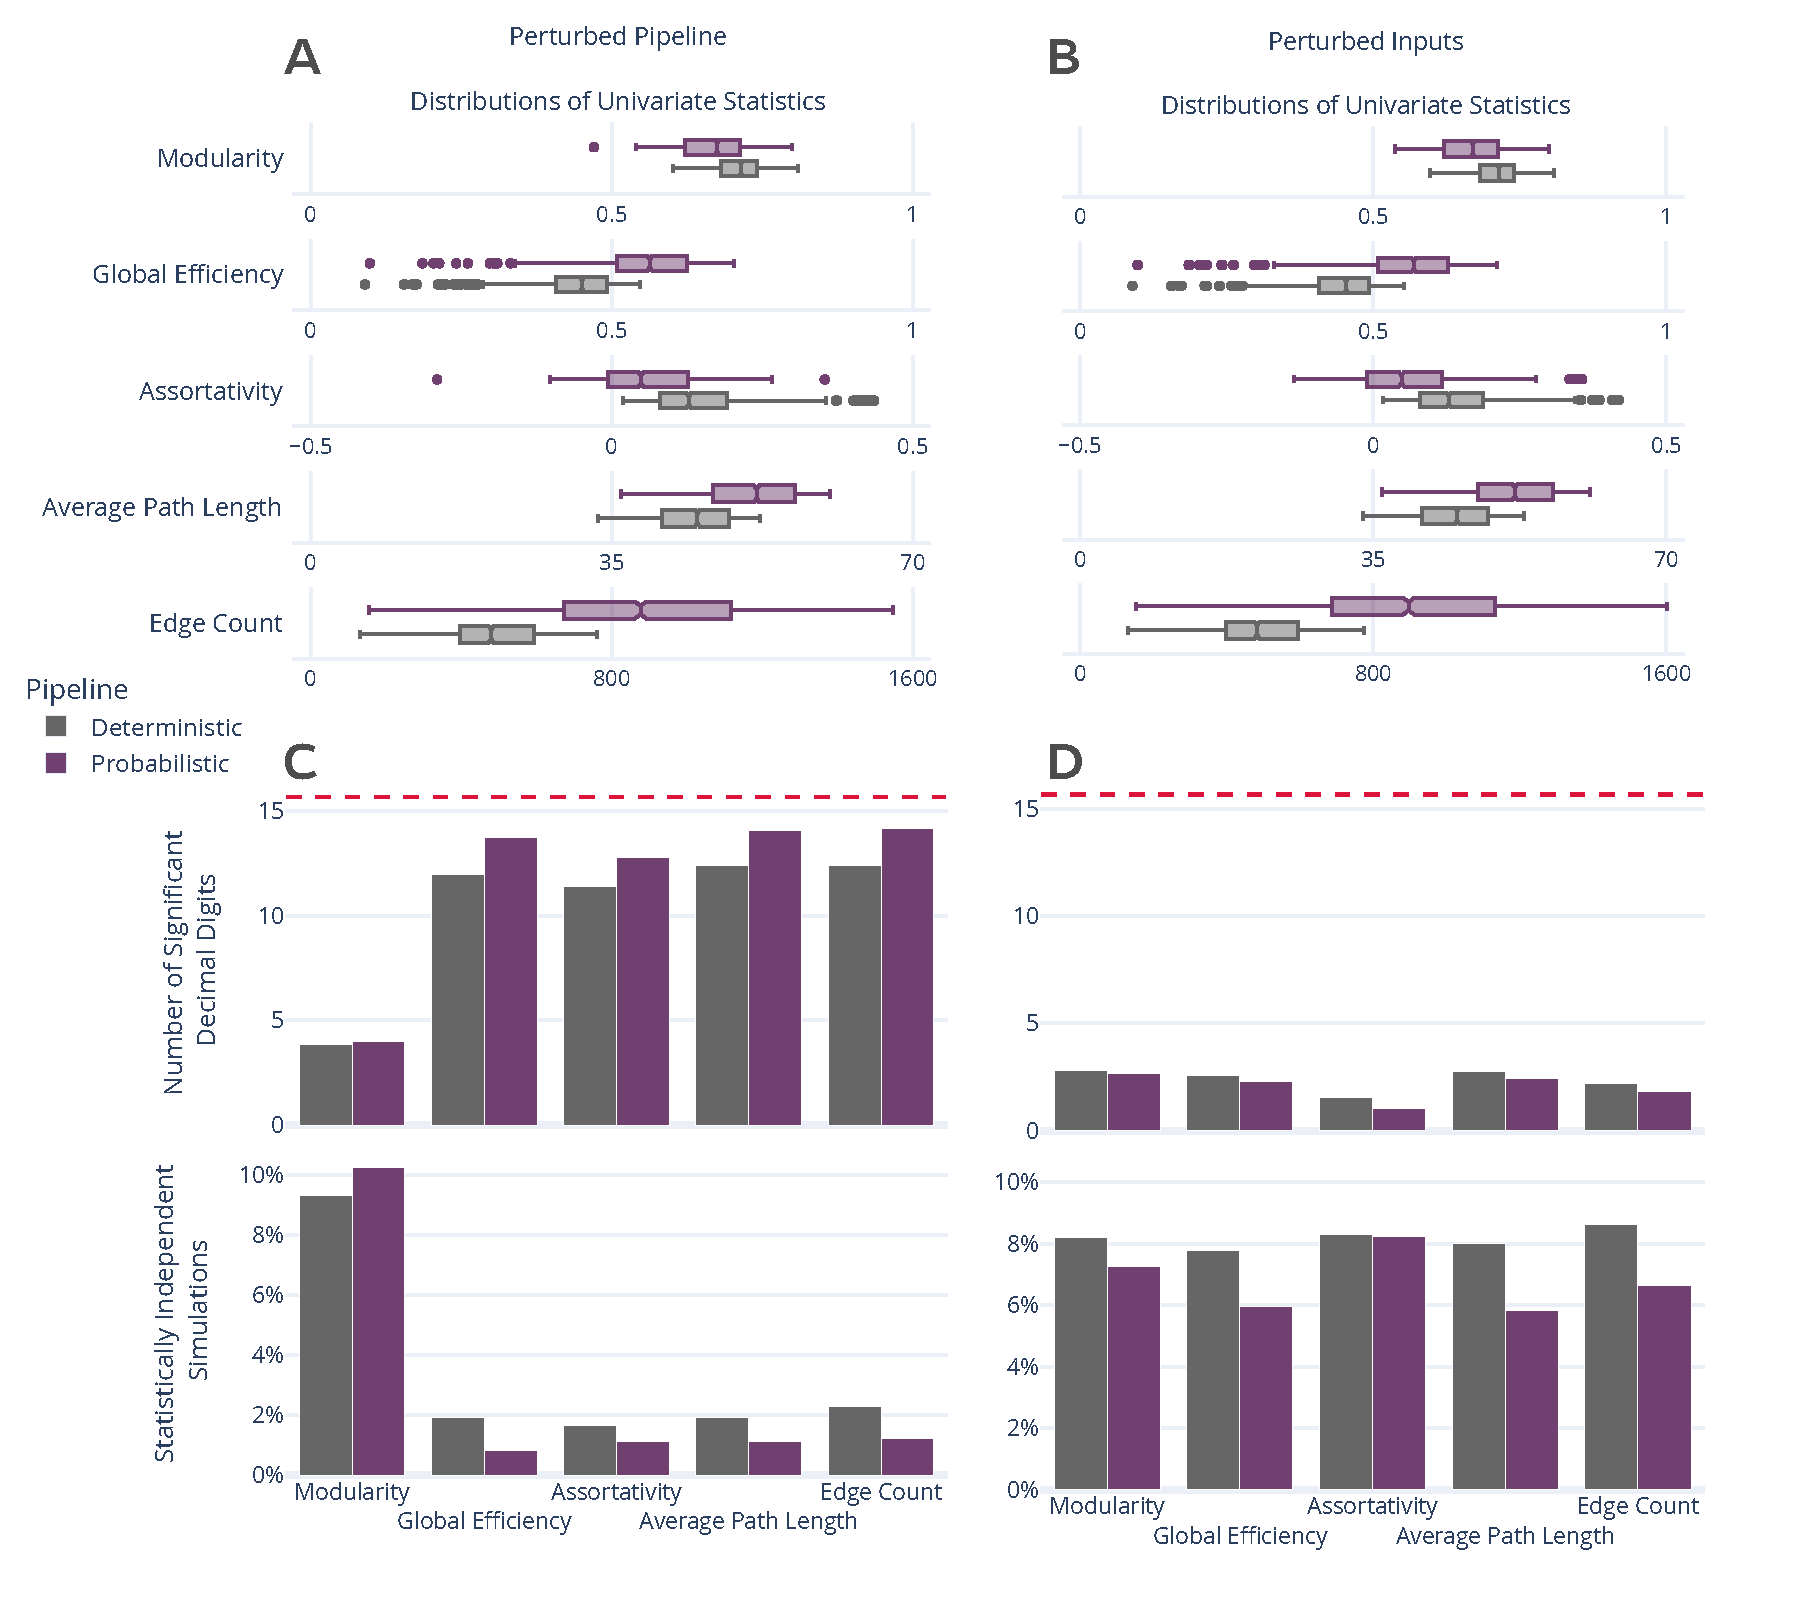
\includegraphics[width=\linewidth]{figures/figS2_univariate_differences.pdf}
\caption{Distribution and stability assessment of univariate graph statistics. (\textbf{A}, \textbf{B}) The
distributions of each computed univariate statistic across all subjects and perturbations for Pipeline and Input
settings, respectively. There was no significant difference between the distributions in A and B. (\textbf{C},
\textbf{D}; top) The number of significant decimal digits in each statistic across perturbations, averaged across
individuals. The dashed red line refers to the maximum possible number of significant digits.
(\textbf{C}, \textbf{D}; bottom) The percentage of connectomes which were deemed significantly different
($p < 0.05$) from the others obtained for an individual.}
\label{sfig:univariate}
\end{figure}


\end{document}
